\documentclass[tikz,border=8pt]{standalone}
% Shared look for every TikZ diagram. Load with % Shared look for every TikZ diagram. Load with % Shared look for every TikZ diagram. Load with \input{../../tools/tikz-style.tex}
\usepackage[T1]{fontenc}
\usepackage{lmodern}
\renewcommand{\sfdefault}{lmr}  % diagrams use the same serif as the text
\usetikzlibrary{arrows.meta, positioning, shapes.geometric, calc, fit, backgrounds}
\definecolor{cblue}{HTML}{4C78A8}
\definecolor{corange}{HTML}{F58518}
\definecolor{cgreen}{HTML}{54A24B}
\definecolor{cred}{HTML}{E45756}
\definecolor{cpurple}{HTML}{B279A2}
\definecolor{cgrey}{HTML}{6B6B6B}
\tikzset{
  every picture/.style={font=\sffamily, line width=1.2pt},
  box/.style={draw=#1, fill=#1!12, rounded corners=4pt, align=center, inner sep=7pt, minimum height=1.1cm},
  box/.default=cgrey,
  arrow/.style={-{Stealth[length=3mm]}, draw=cgrey, line width=1.4pt},
  title/.style={font=\sffamily\bfseries\Large},
  note/.style={font=\sffamily\small, text=cgrey, align=center},
}
\AtBeginDocument{\hyphenpenalty=10000 \exhyphenpenalty=10000}

\usepackage[T1]{fontenc}
\usepackage{lmodern}
\renewcommand{\sfdefault}{lmr}  % diagrams use the same serif as the text
\usetikzlibrary{arrows.meta, positioning, shapes.geometric, calc, fit, backgrounds}
\definecolor{cblue}{HTML}{4C78A8}
\definecolor{corange}{HTML}{F58518}
\definecolor{cgreen}{HTML}{54A24B}
\definecolor{cred}{HTML}{E45756}
\definecolor{cpurple}{HTML}{B279A2}
\definecolor{cgrey}{HTML}{6B6B6B}
\tikzset{
  every picture/.style={font=\sffamily, line width=1.2pt},
  box/.style={draw=#1, fill=#1!12, rounded corners=4pt, align=center, inner sep=7pt, minimum height=1.1cm},
  box/.default=cgrey,
  arrow/.style={-{Stealth[length=3mm]}, draw=cgrey, line width=1.4pt},
  title/.style={font=\sffamily\bfseries\Large},
  note/.style={font=\sffamily\small, text=cgrey, align=center},
}
\AtBeginDocument{\hyphenpenalty=10000 \exhyphenpenalty=10000}

\usepackage[T1]{fontenc}
\usepackage{lmodern}
\renewcommand{\sfdefault}{lmr}  % diagrams use the same serif as the text
\usetikzlibrary{arrows.meta, positioning, shapes.geometric, calc, fit, backgrounds}
\definecolor{cblue}{HTML}{4C78A8}
\definecolor{corange}{HTML}{F58518}
\definecolor{cgreen}{HTML}{54A24B}
\definecolor{cred}{HTML}{E45756}
\definecolor{cpurple}{HTML}{B279A2}
\definecolor{cgrey}{HTML}{6B6B6B}
\tikzset{
  every picture/.style={font=\sffamily, line width=1.2pt},
  box/.style={draw=#1, fill=#1!12, rounded corners=4pt, align=center, inner sep=7pt, minimum height=1.1cm},
  box/.default=cgrey,
  arrow/.style={-{Stealth[length=3mm]}, draw=cgrey, line width=1.4pt},
  title/.style={font=\sffamily\bfseries\Large},
  note/.style={font=\sffamily\small, text=cgrey, align=center},
}
\AtBeginDocument{\hyphenpenalty=10000 \exhyphenpenalty=10000}

\begin{document}
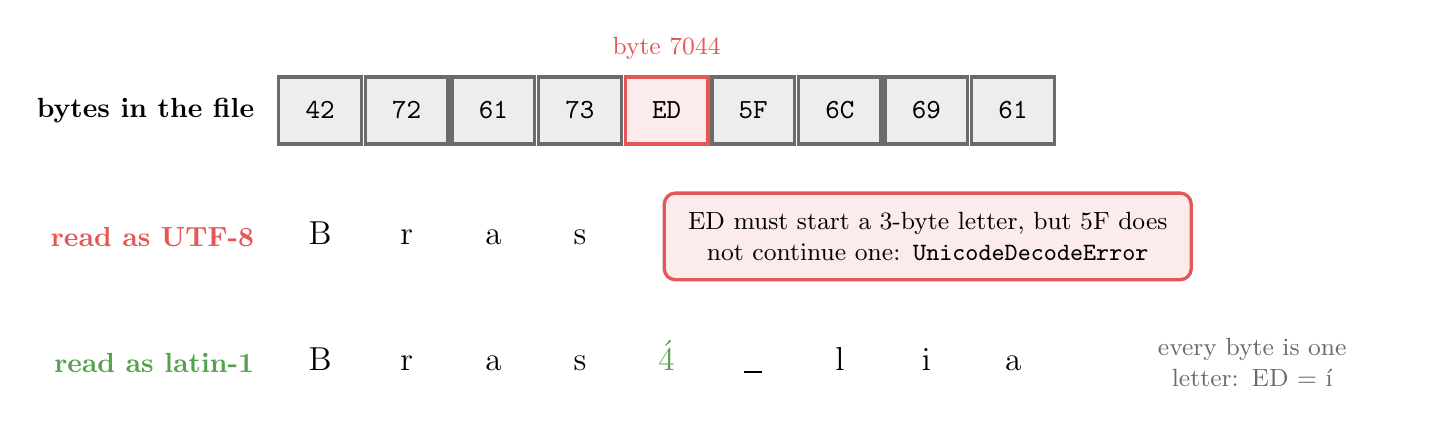
\begin{tikzpicture}[b/.style={draw=#1, fill=#1!12, minimum width=1.05cm, minimum height=0.85cm, font=\ttfamily},
                    ch/.style={minimum width=1.05cm, font=\large, text height=1.8ex, text depth=0.5ex}]
  \node[anchor=east, font=\bfseries] at (-0.2,0) {bytes in the file};
  \foreach \h/\c [count=\i from 0] in {42/cgrey, 72/cgrey, 61/cgrey, 73/cgrey, ED/cred, 5F/cgrey, 6C/cgrey, 69/cgrey, 61/cgrey}
    \node[b=\c] (b\i) at (1.1*\i+0.5,0) {\h};
  \node[note, above=2pt of b4, text=cred] {byte 7044};
  % UTF-8 reading
  \node[anchor=east, font=\bfseries, text=cred] at (-0.2,-1.6) {read as UTF-8};
  \foreach \c [count=\i from 0] in {B,r,a,s} \node[ch] at (1.1*\i+0.5,-1.6) {\c};
  \node[box=cred, anchor=west, text width=6.2cm, font=\small] at (4.85,-1.6) {ED must start a 3-byte letter, but 5F does not continue one: \texttt{UnicodeDecodeError}};
  % latin-1 reading
  \node[anchor=east, font=\bfseries, text=cgreen] at (-0.2,-3.2) {read as latin-1};
  \foreach \c/\k [count=\i from 0] in {B/black,r/black,a/black,s/black,í/cgreen,{\rule[-0.2ex]{0.55em}{0.9pt}}/black,l/black,i/black,a/black} \node[ch, text=\k] at (1.1*\i+0.5,-3.2) {\c};
  \node[note, anchor=west, text width=3.6cm] at (10.4,-3.2) {every byte is one letter: ED = í};
\end{tikzpicture}
\end{document}
